\documentclass{article}

% required 
\usepackage[hyphens]{url} % this wraps my URL versus letting it spill across the page, a bad habit LaTeX has
\usepackage{Sweave}
\usepackage{graphicx}% Required for including images
\usepackage{natbib}
\usepackage{amsmath}
\usepackage{textcomp}%among other things, it allows degrees C to be added
\usepackage{float}% Required for the [H] placement specifier
\usepackage[utf8]{inputenc} % allow funny letters in citations 
\usepackage[nottoc]{tocbibind} %should add Re fences to the table of contents?
\usepackage{amsmath} % making nice equations 
\usepackage{listings} % add in stan code
\usepackage{xcolor}
\usepackage{capt-of}%allows me to set a caption for code in appendix 
\usepackage[export]{adjustbox} % adding a box around a map
\usepackage{lineno}
%\linenumbers
% recommended! Uncomment the below line and change the path for your computer!
% \SweaveOpts{prefix.string=/Users/Lizzie/Documents/git/teaching/demoSweave/Fig.s/demoFig, eps=FALSE} 
%put your Fig.s in one place! Also, note that here 'Fig.s' is the folder and 'demoFig' is what each 
% Fig. produced will be titled plus its number or label (e.g., demoFig-nqpbetter.pdf')
% make your captioning look better
\usepackage[small]{caption}
\usepackage{caption}% Required for custom caption formatting
\usepackage{xr-hyper} %refer to Fig.s in another document
\usepackage{hyperref}




\setlength{\captionmargin}{30pt}
\setlength{\abovecaptionskip}{0pt}
\setlength{\belowcaptionskip}{10pt}

% optional: muck with spacing
\topmargin -1.5cm        
\oddsidemargin 0.5cm   
\evensidemargin 0.5cm  % same as odd side margin but for left-hand pages
\textwidth 16.59cm
\textheight 23.94cm 
% \renewcommand{\baselinestretch}{1.5} % 1.5 lines between lines
\parindent 0pt		  % sets leading space for paragraphs
% optional: cute, fancy headers
\usepackage{fancyhdr}
\pagestyle{fancy}
%\fancyhead[LO]{Frederik Baumgarten}
%\fancyhead[RO]{Research Proposal}
% more optionals! %
\usepackage{booktabs} %clean and professional look for tables

\graphicspath{ {/Users/frederik/github/PhaenoFlex_clean/docs/figs/} }% tell latex where to find figures 
% \setlength{\parindent}{2em} % Sets the paragraph indentation to 2 em spaces
\begin{document}
	%	\renewcommand{\bibname}{References}%names reference list 
	
	
	\title{Scientific final report for project PhaenoFlex: \\
		Influence of the timing of stress and stimuli on growth performance, phenological development and survival of temperate trees	%(my favourite)
	} 
	
	\author{Frederik Baumgarten\textsuperscript{1,2}}
	\maketitle
	
	$^1$ Department of Forest and Conservation, Faculty of Forestry, University of British Columbia, Vancouver, Canada. \\
	$^2$ Department of Environmental Science-Botany, University of Basel, Basel, Switzerland. \\
	
	Postdoc.mobility, project number: P500PB\_210943\\
	%	\date{\today}
	\section*{Summary} %10-15
	To which degree plants and forests are affected by environmental stress may depend largely on the timing of the event and at which developmental stage plants are hit. This study investigates the phenotypic plasticity of growth processes. This study explores the impact of three controlled drought and defoliation treatments using 630 saplings of six species. Results indicate that defoliation imposes a stronger negative impact on tree growth than drought, particularly affecting determinate species reliant on pre-formed leaves. The timing of stress events significantly influences biomass accumulation, with the most pronounced effects observed at the end of June during peak growth. Indeterminate species that are able to form new tissue in the current year, may cope better with increased frequency of environmental stress by shifting their growth activities towards the season's end. This functional trait may be crucial for adaptation in future climatic conditions. 
	Our findings also highlight that the effects of environmental stress might not become evident until the following year, rather than in the year they occur.
	
	\section*{1. Project description}
	
	\subsection*{1.1 Research questions and main results}
	\textbf{Study Species and Site:} \\
	This project investigated the phenotypic plasticity of growth in response to environmental stress, namely drought and defoliation. Specifically we addressed the following research questions:\\
	
	1. What are the relative impacts of sink and source limitations caused by drought and defoliation events on growth performance?\\
	2. Does timing of similar stress treatments matter?\\
	3. Are their functional traits explaining species-specific differences in the observed responses?\\
	
	This study examined the diverse responses of tree species to environmental stress by focusing on saplings from six species across different plant families, including both coniferous evergreens and broadleaved deciduous types. The chosen species were \textit{Pinus contorta}, \textit{Sequoia sempervirens}, \textit{Prunus virginiana}, \textit{Acer macrophyllum}, \textit{Betula papyrifera}, and \textit{Quercus garryana}. These species naturally thrive along the Pacific west coast, where our experiments took place at the University of British Columbia in Vancouver, Canada. 
	
	Each sapling was subjected to one of six treatments (plus a control): three different drought timings and three defoliation events with a total of 105 saplings per species (6 treatments plus control * 15 replicates * 6 species). 
	
	Drought treatments were conducted in climate chambers where temperatures were maintained at 30°C during the day and 20°C at night. Drought conditions were monitored by observing soil moisture and signs of stress, such as leaf desiccation. Defoliation treatments mimicked leaf loss from natural causes by trimming unfolded leaves. Drought and defoliation treatments were performed on the same three occasions: After leaf-out (species-specific), 23. June and 1. August.  
	
	Throughout the study, phenological developments of apical and radial meristems were monitored. Devices like magnetic dendrometers captured diameter fluctuations without damaging the saplings. Upon reaching full dormancy, saplings were harvested, dried, and segmented for biomass and wood anatomical analysis. The pinning technique was used to set marker in time for later reconstruction of wood formation prior and after treatments. 	\\
	
	
	\textbf{Apical shoot growth:}
	Shoot elongation showed species-specific patterns with distinct determinate to indeterminate behaviour. Acer, Prunus and Quercus ceased apical shoot growth shortly after preformed tissue in buds was elongated (few weeks after budburst. In contrast Betula, Sequoia and to some extent Pinus showed continues growth throughout the season, in some cases until low temperature in autumn induced senescence of the foliage.\\
	\begin{figure}[H]
		\centering
		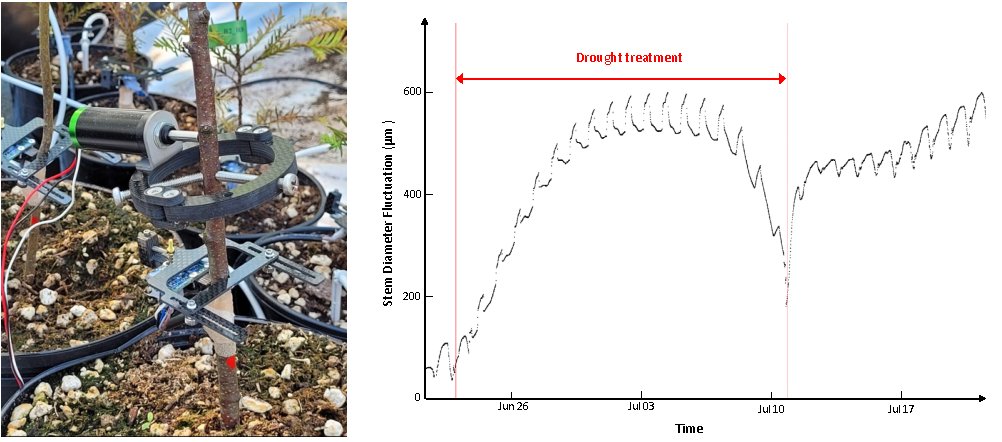
\includegraphics[width=0.8\linewidth, height=0.6\textheight, keepaspectratio]{dendrometer_graph.pdf} 
		\caption{Left: Newly developed magnetic dendrometer (at the stem base) were used to monitor radial growth in a 15 min interval. Their performance was compared to classical point dendrometers (upper part of the stem). Right: Example of the changes in stem diameter of a Bigleaf maple sapling during a drought treatment and subsequent recovery phase.}
		\label{fig:dendrometer_graph}
	\end{figure}
	
	\textbf{Radial cambial growth:}
	The specifically designed magnetic dendrometers performed well and yielded very accurate and comparable results compared to standard point dendrometer (see Fig. \ref{fig:dendrometer_graph}). Measurements during and after drought treatments indicated strong tree water deficits with strong stem shrinkage and almost no recovery during the night (Fig. \ref{fig:dendrometer_graph}). Together with soil moisture measurements this is prove of severe drought conditions. Nevertheless most individuals showed strong recovery after drought stress release. 	\\
	
	
	\textbf{Treatment effects on biomass:}
	Total biomass at the end of the growing seasons was lowest for saplings of all species that were defoliated --- surprisingly even lower than drought-exposed saplings. Although saplings needed a longer recovery from defoliation than from drought stress, Quercus as a fully recovering species that quickly re-flushes from dormant spare buds, showed most reduced biomass compared to control saplings (Fig. \ref{fig:biomass_post_treat_sub}).
	Comparing different timings of drought and defoliation events revealed that biomass accumulation and therefore growth is mostly sensitive to stress around the summer solstice. However, drought had also little effects on biomass just after leaf-out and was negligible in August. Defoliation had even a small positive effect on biomass accumulation in Prunus, Betula and Pinus. Presumably these species were able to compensate later in the season as was observed by a later date of senescence (data not shown here).
	\\
	
	\begin{figure}[H]
		\centering
		\begin{minipage}[t]{0.5\textwidth} % Adjust the width to fit your needs
			\vspace{0pt} % Align the top of minipage with the top of the figure
			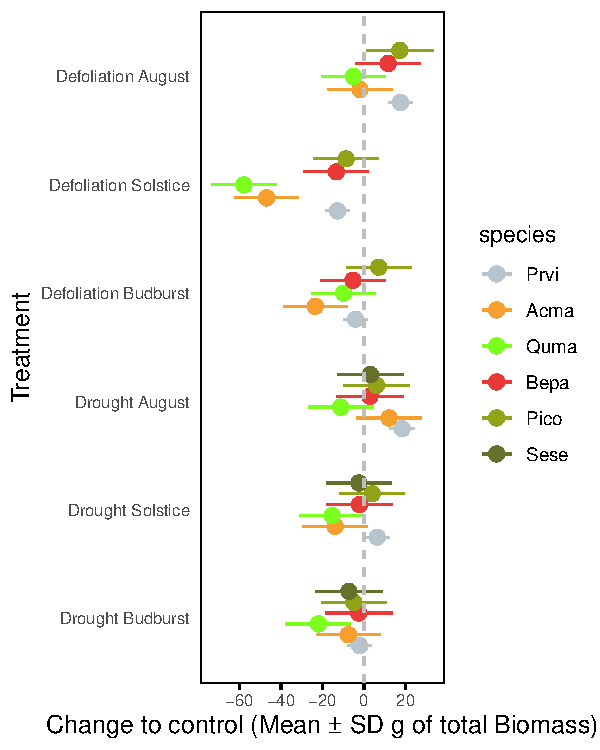
\includegraphics[width=\linewidth, height=0.5\textheight, keepaspectratio]{biomass_post_treat_sub.pdf}
		\end{minipage}%
		\hfill
		\begin{minipage}[t]{0.5\textwidth} % Adjust the width to matc the figure minipage
			\vspace{0pt} % Align the top of minipage with the top of the figure
			\caption{Effect size in g of biomass compared to control sapling when exposed to defoliation or drought treatments on 3 occasions. Colors represent the six study species. Shown are means±SD of the posteriors. Prvi: Prunus; Acma: Acer; Quma: Quercus; Bepa: Betula; Pico: Pinus; Sese: Sequoia.}
			\label{fig:biomass_post_treat_sub}
		\end{minipage}
	\end{figure}
	
	
	%\textbf{Wood anatomy}
	%Data processing is still under way due to the underestimated time required.
	
	\begin{figure}[H]
		\centering
		\begin{minipage}[t]{0.6\textwidth} % Adjust the width to fit your needs
			\vspace{0pt} % Align the top of minipage with the top of the figure
			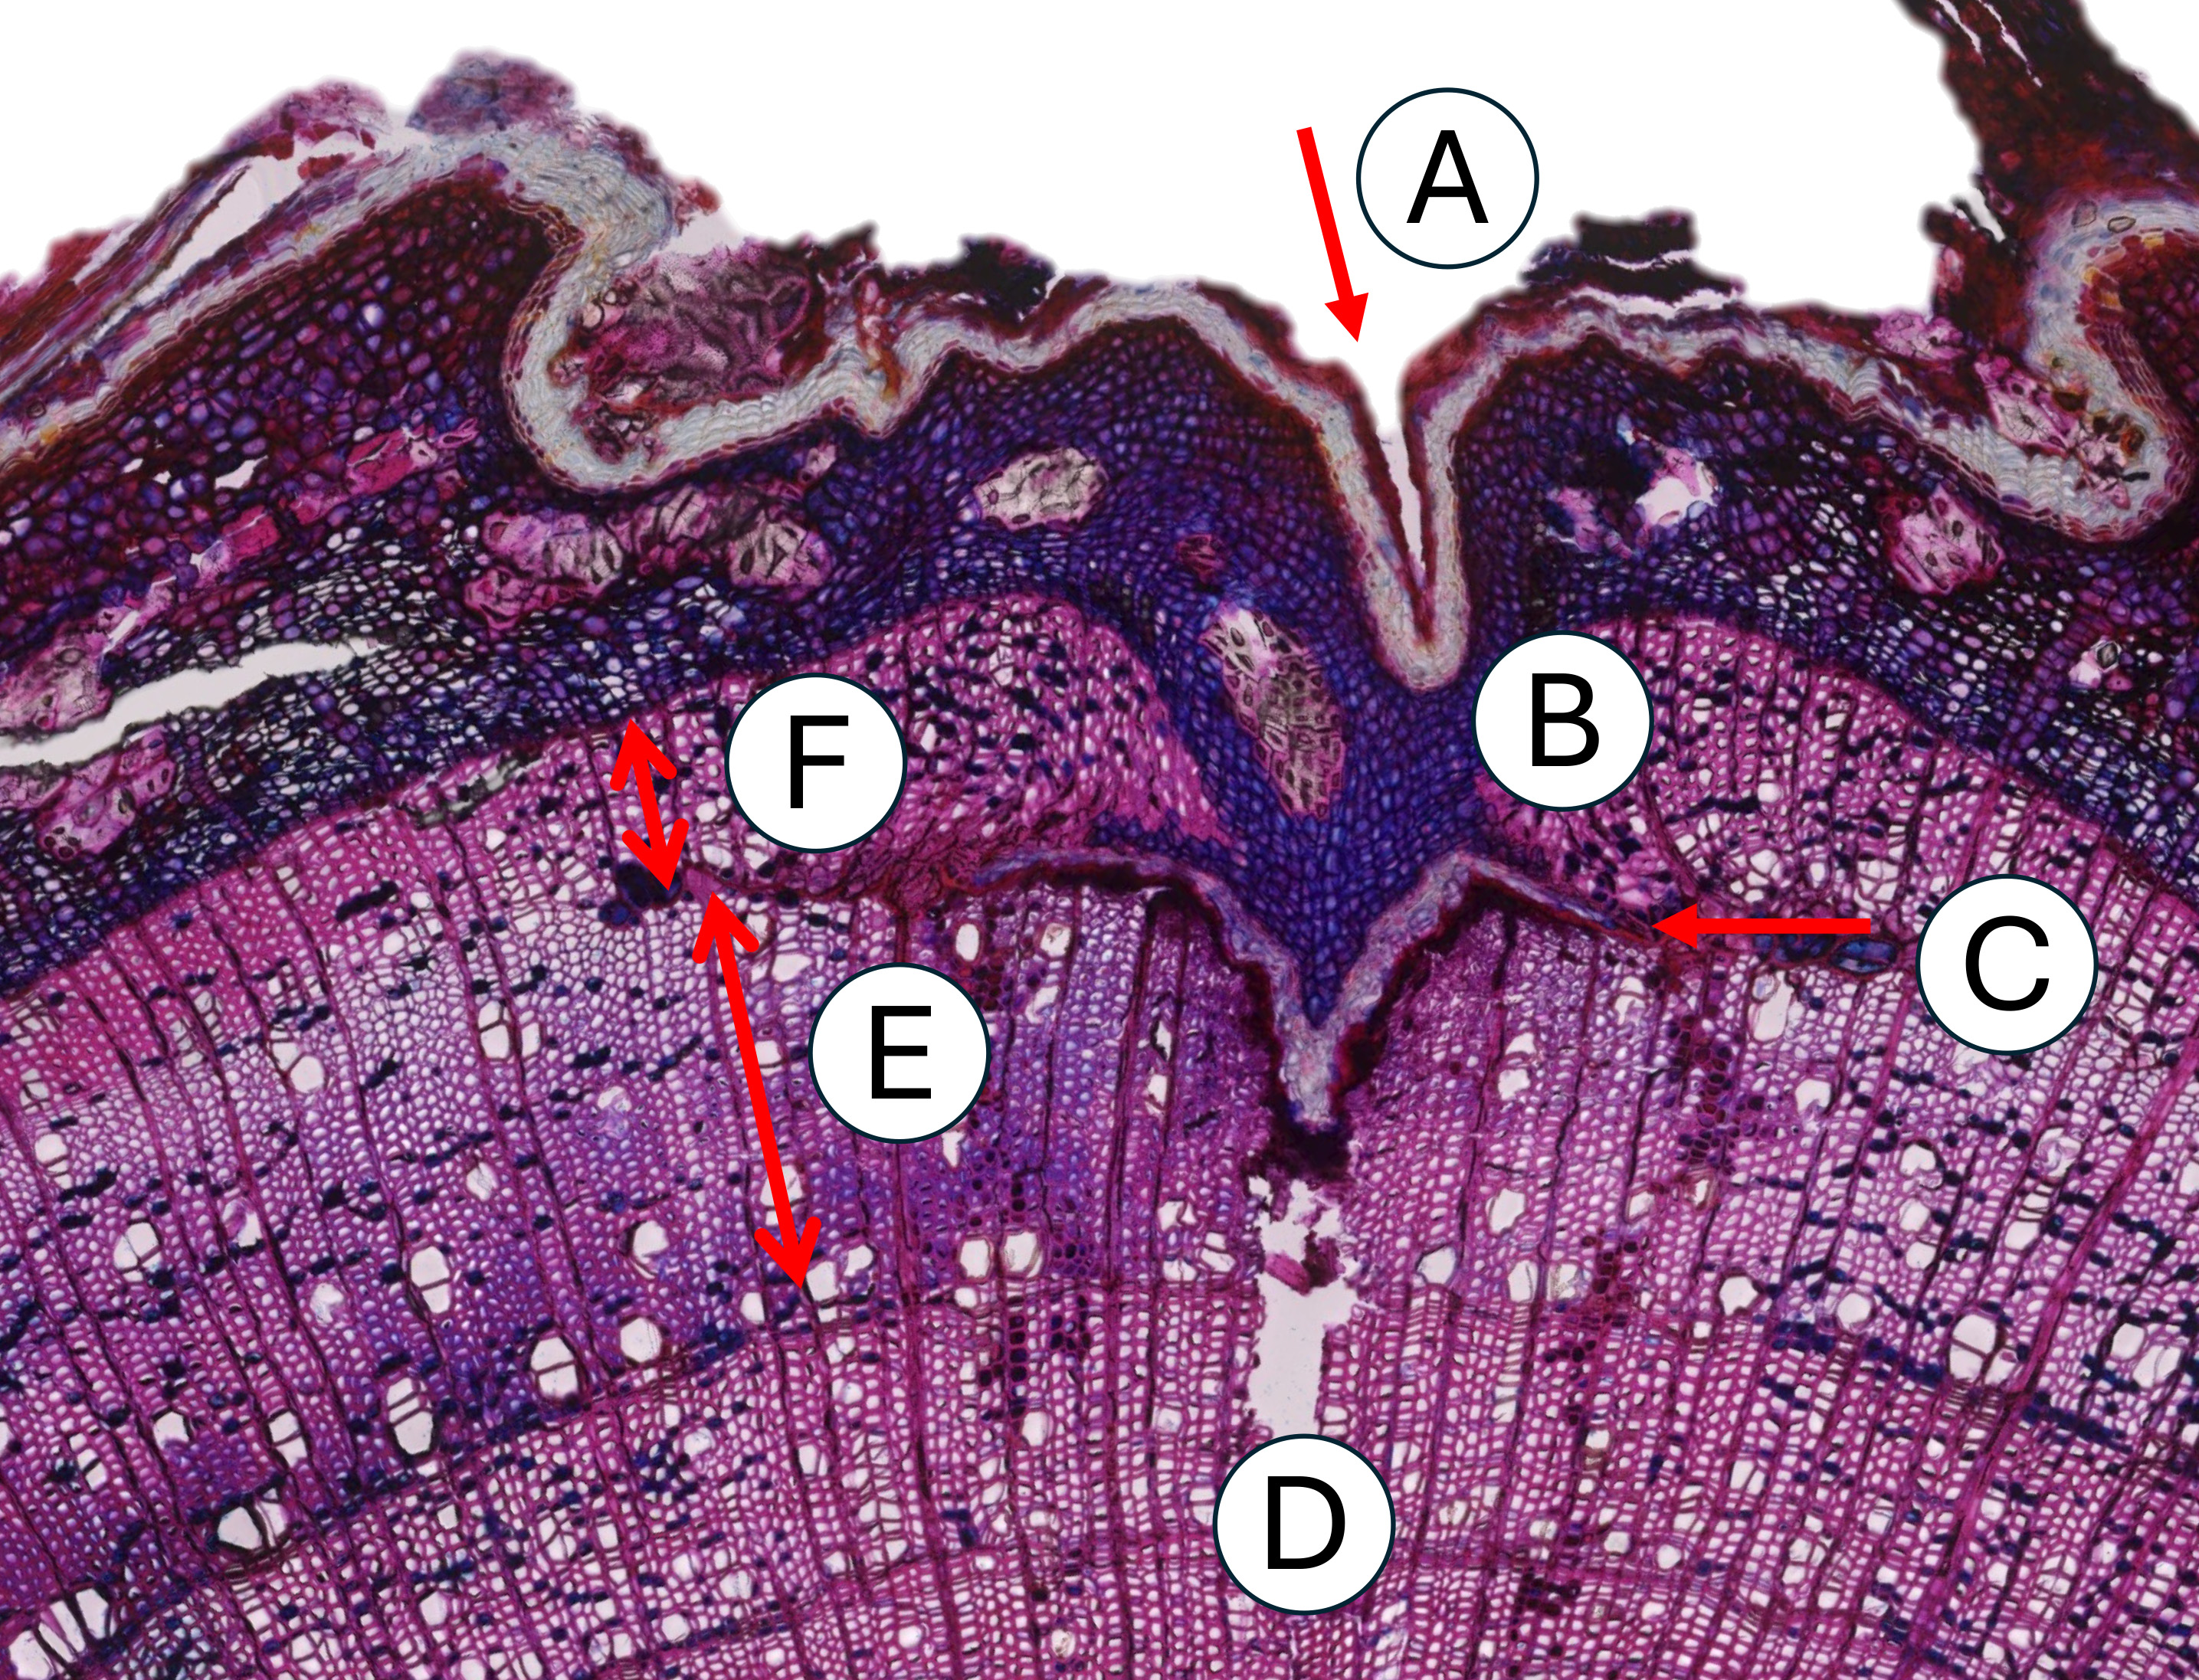
\includegraphics[width=0.8\linewidth, height=0.6\textheight, keepaspectratio]{pinning_closup_x2.jpg}
		\end{minipage}%
		\hfill
		\begin{minipage}[t]{0.4\textwidth} % Adjust the width to matc the figure minipage
			\vspace{0pt} % Align the top of minipage with the top of the figure
			\caption{Cross-section of \textit{Quercus garryana} depicting the reaction caused by the pinning. A: pinning hole with bark and phloem cells; B: zone of irritated cambial cells surrounding the pinning hole (callose tissue); C: border of cambium at the time of pinning; D: Pinning hole penetrating into the xylem cells that were already formed at the time of pinning; E: xylem cells formed prior to pinning; F: xylem cells formed after pinning.}
			\label{fig:pinning_closup_x2}
		\end{minipage}
	\end{figure}
	
	
	\subsection*{Conclusions}
	Preliminary results indicate that defoliation has a stronger negative impact on growth than drought after one growing season. Moreover, effects of stress timing on biomass accumulation matters and is most pronounced in end of June when growth is commonly observed to peak. The pronounced effect of leaf removal, despite fast recovery in most species is surprising because trees are thought to be sink-limited: cell division and maturation are thought to be the most critical and sensitive physiological processes with sugar assimilates often used from reserves. Our data indicate that the formation of new tissue is indeed dependent on fresh assimilates. Moreover, determinate species, that rely on pre-build leaves for the entire season only, appear to be most affected from defoliation events. Indeterminate growing species, in contrast, may compensate stress episodes by prolonging or shifting their growth phenology. Such a phenotypic plasticity may become crucial in a climate with increased frequency of environmental stress and should be further investigated as an important functional trait.\\
	
	Our results also emphasize that the effects of environmental stress may not become apparent in the current year but could rather manifest in the subsequent year. Determinate species, in particular, are likely to experience reduced performance in the following year, as their entire next year's foliage is formed in the current year, eventually under poor conditions. This in turn may largely define the growth potential in the upcoming year.\\
	
	
	\subsection*{1.2 Changes to the planned research project}
	The study was carried out as planned. Due to the time consuming processing of wood anatomical samples the whole schedule got delayed. \\
	
	\subsection*{1.3 Planned publications}
	
\begin{table}[H]
	\caption{Scientific papers that were funded under the period of the applicant's postdoc.mobility funding}
	\centering
	\begin{tabular}{|p{8.7cm}|p{2cm}|p{5.0cm}|}
		\hline
		\textbf{Title} & \textbf{Status} & \textbf{Description} \\ 
		\hline
		Phenological plasticity: shifting growth and developmental phases ofNorth American tree species in response to environmental stressors & In prep & data-paper of the main experiment \\ 
		\hline
		Invest now, get paid later?Growth strategies to cope with environmental stress and benefit from extendedgrowing seasons in a future climate & Submitted & conceptual review paper of a major research finding \\ 
		\hline
		Why longer seasons with climate change may not increase tree growth. & Submitted & meta-analysis \\ 
		\hline
		The power of simulating data: a tool to designexperiments, understand data limitations and improve scientific reasoning & In prep & conceptual paper of why and how science can do even better\\ 
		\hline
	\end{tabular}
\end{table}
	
	This finding has inspired one follow-up project: an experiment was launched in 2024 to investigate how warming in spring and/or autumn affects growth performance not only in the current but also in the following year (carry over effect). \\
	Part of this work was presented at ESA, Longbeach, CA and EGU, Vienna. 
	
	
	%\section*{stuff I did't find place yet}
	
	
	
	
	
	\bibliography{refs_phaenoflex}
	\bibliographystyle{ecolett}
	
	
	
	
	
	
\end{document}
